\begin{figure}
\centering
\begin{tabular}{lc}
    \rotatebox[origin=l]{90}{\bf \quad\quad$k$-Median} &
    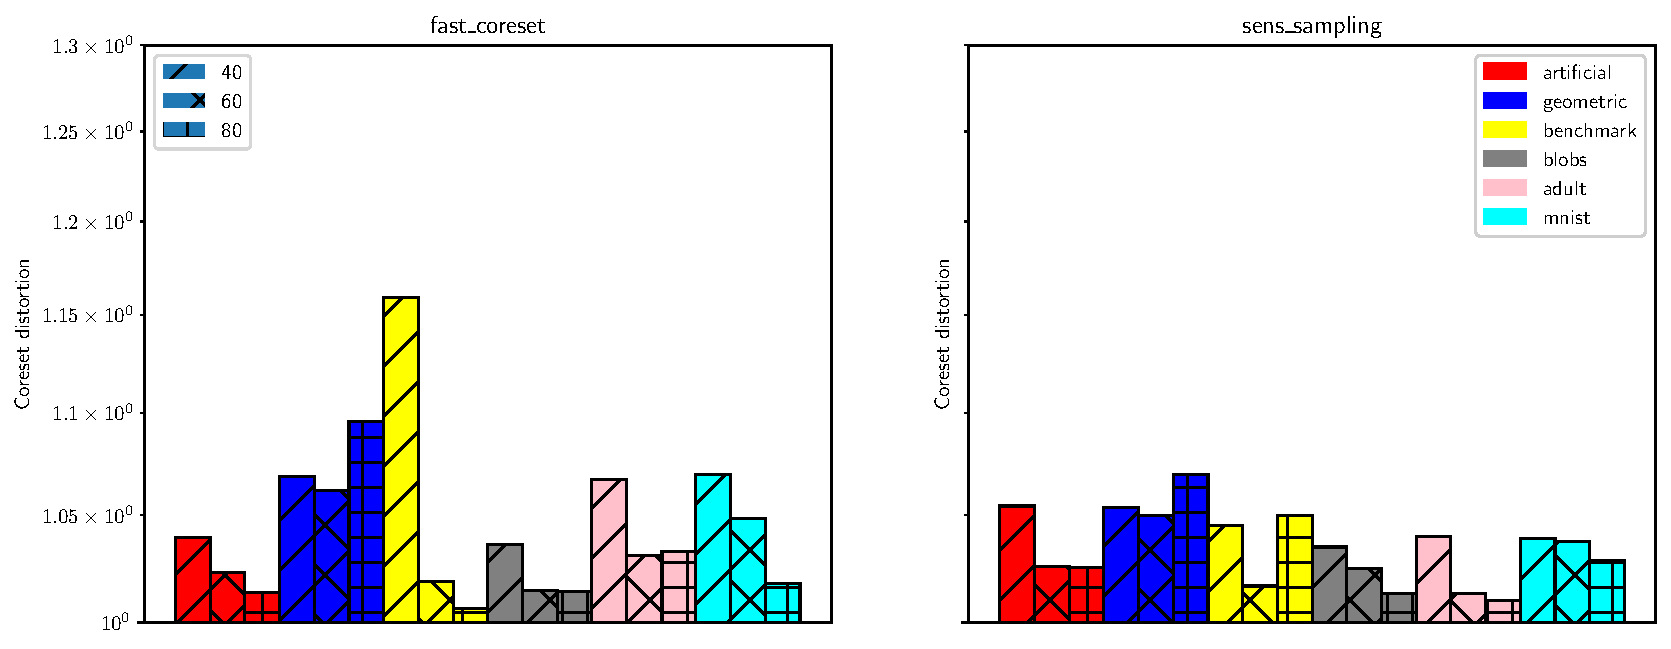
\includegraphics[width=.9\linewidth]{images/1/coreset_distortion-m_scalar_for_sens_sampling.pdf} \\

    \rotatebox[origin=l]{90}{\bf \quad\quad$k$-Means} &
    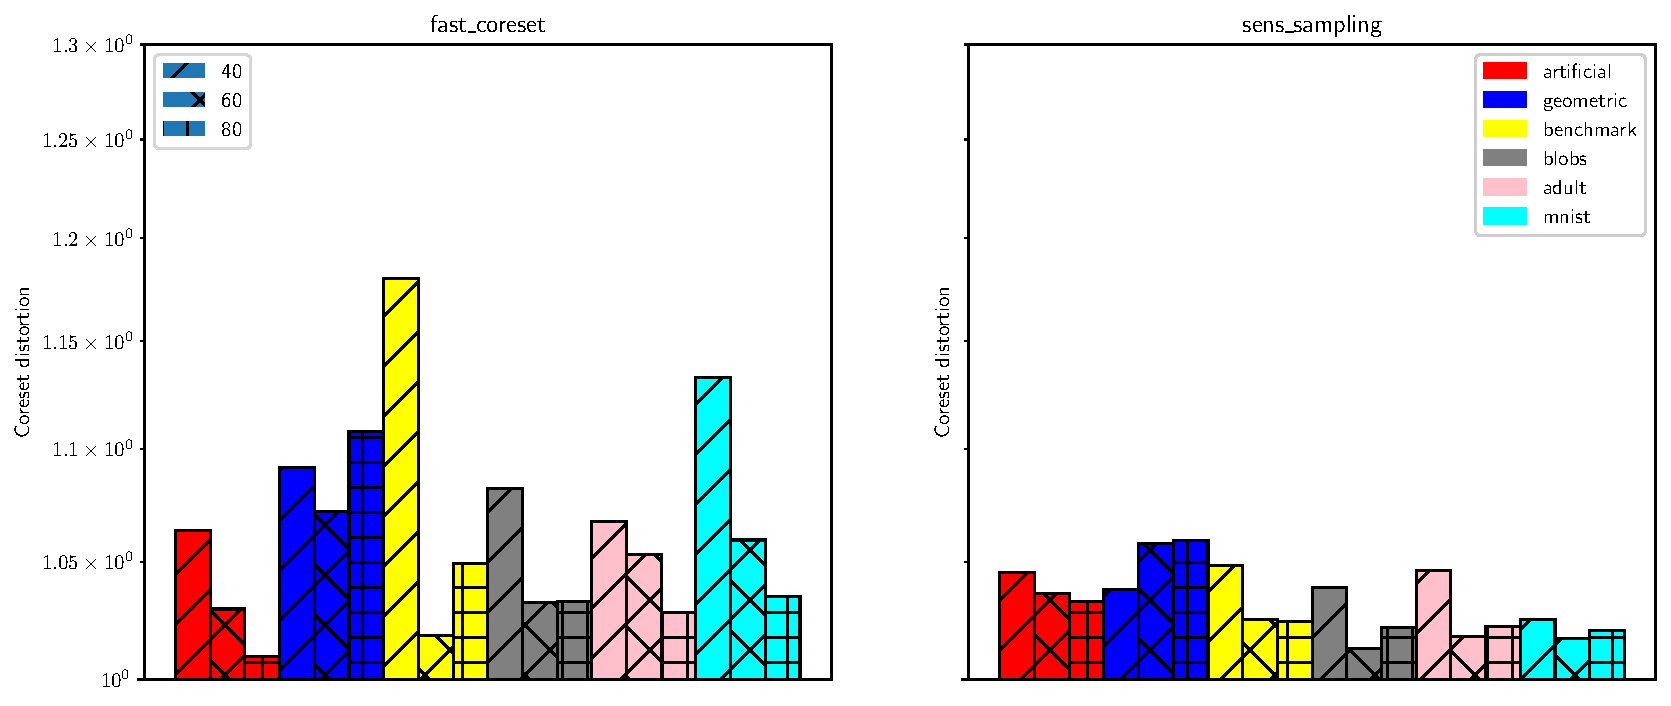
\includegraphics[width=.9\linewidth]{images/2/coreset_distortion-m_scalar_for_sens_sampling.pdf}
\end{tabular}
\caption{The effect of the coreset size on the distortion metric for sensitivity sampling approaches.
We point out that all distortion values are well below $\varepsilon = 0.2$.
Thus, for sufficient coreset sizes ($m\text{-scalar}\geq60$), there does not seem to be a meaningful difference between using Fast-$k$-means++ vs. regular $k$-means++.}
\label{fig:coreset_size_on_sens_quality}
\end{figure}
